\documentclass{beamer}
\usetheme{Madrid}
\usecolortheme{default}
\usepackage[utf8]{inputenc}
\usepackage[T1]{fontenc}
\usepackage{lmodern}
\usepackage{amsmath,amssymb}
\usepackage{bm}
\usepackage{graphicx}
\usepackage{tikz}
\usetikzlibrary{arrows.meta,positioning,calc,shapes}
\usepackage{booktabs}
\usepackage{hyperref}
\usepackage{xcolor}

% Custom Colors
\definecolor{rsvpblue}{RGB}{0,102,204}
\definecolor{rsvpred}{RGB}{204,0,0}
\definecolor{rsvpgray}{RGB}{100,100,100}
\definecolor{rsvpgreen}{RGB}{0,153,0}

% Title
\title{\Large\textbf{Entropic Redshift and the RSVP Stack:\\A Unified Field Ontology for Cosmos, Mind, and Society}}
\author{Flyxion}
\institute{Independent Researcher}
\date{\today}

% Custom Commands
\newcommand{\stacklayer}[5]{
  \node[draw,rounded corners,fill=#1,minimum height=1cm,minimum width=2.5cm] (#2) {#3};
  \node[above=0.1cm of #2, font=\small] {#4};
  \node[below=0.1cm of #2, font=\scriptsize] {#5};
}

\begin{document}

% ------------------------------------------------------------------
% Slide 1: Title
% ------------------------------------------------------------------
\begin{frame}
\titlepage
\begin{center}
\vspace{1em}
\textit{“The universe is not made of things, but of processes.”} — A. N. Whitehead
\end{center}
\end{frame}

% ------------------------------------------------------------------
% Slide 2: The Problem
% ------------------------------------------------------------------
\begin{frame}{The Fragmentation of Reality}
\begin{columns}
\begin{column}{0.33\textwidth}
\textbf{Cosmology}\\[0.5em]
\begin{itemize}
\item Metric expansion
\item Dark energy
\item Redshift = $z_\Lambda$
\end{itemize}
\end{column}
\begin{column}{0.33\textwidth}
\textbf{Cognition}\\[0.5em]
\begin{itemize}
\item Symbolic computation
\item Free energy principle
\item Sparse coding
\end{itemize}
\end{column}
\begin{column}{0.33\textwidth}
\textbf{Society}\\[0.5em]
\begin{itemize}
\item Institutions as contracts
\item Memetic evolution
\item Boundary rituals
\end{itemize}
\end{column}
\end{columns}
\vspace{1em}
\centering
\alert{No shared dynamical language.}
\end{frame}

% ------------------------------------------------------------------
% Slide 3: The RSVP Stack
% ------------------------------------------------------------------
\begin{frame}{The RSVP Stack: Unified Field Ontology}
\begin{center}
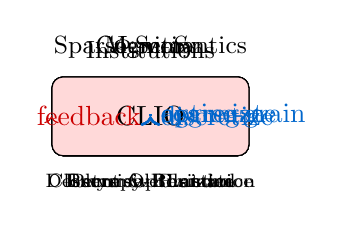
\begin{tikzpicture}[node distance=10mm]
  \stacklayer{gray!20}{rsvp}{RSVP}{$\Phi,\mathbf{v},S$}{Physical Plenum}
  \stacklayer{blue!15}{ebssc}{EBSSC}{Sparse Semantics}{Entropy-Bounded}
  \stacklayer{green!15}{sphere}{Spherepop}{Institutions}{Closure \& Resistance}
  \stacklayer{orange!15}{tartan}{TARTAN}{Memory}{Recursive Lattice}
  \stacklayer{red!15}{clio}{CLIO}{Cognition}{Descent Optimization}

  \draw[->,thick,rsvpblue] (rsvp) -- (ebssc) node[midway,right] {coarse-grain};
  \draw[->,thick,rsvpblue] (ebssc) -- (sphere) node[midway,right] {aggregate};
  \draw[->,thick,rsvpblue] (sphere) -- (tartan) node[midway,right] {discretize};
  \draw[->,thick,rsvpblue] (tartan) -- (clio) node[midway,right] {optimize};
  \draw[->,dashed,rsvpred] (clio.west) to[bend left=60] (rsvp.west) node[midway,left] {feedback};
\end{tikzpicture}
\end{center}
\alert{All layers = functors on same field dynamics.}
\end{frame}

% ------------------------------------------------------------------
% Slide 4: Core Equations
% ------------------------------------------------------------------
\begin{frame}{RSVP Field Equations}
From variational principle:
\[
\mathcal{A} + \mathcal{D} = \int \left( \frac{1}{2}\|\mathbf{v}\|^2 + \frac{1}{2}\Phi^2 - S \right) + \text{dissipation}
\]
\begin{align*}
\partial_t \Phi &= -\nabla\cdot(\Phi \mathbf{v}) + \kappa_\Phi \Delta \Phi \\
\partial_t \mathbf{v} &= -(\mathbf{v}\cdot\nabla)\mathbf{v} - \nabla \Phi + \kappa_v \Delta \mathbf{v} \\
\partial_t S &= \sigma + \kappa_S \Delta S - \lambda S
\end{align*}
\vspace{0.5em}
\begin{block}{Interpretation}
\begin{itemize}
\item $\Phi$: \alert{semantic density}
\item $\mathbf{v}$: \alert{agency flow}
\item $S$: \alert{entropic cost}
\end{itemize}
\end{block}
\end{frame}

% ------------------------------------------------------------------
% Slide 5: Entropic Redshift
% ------------------------------------------------------------------
\begin{frame}{Entropic Redshift: No Expansion Needed}
\[
\boxed{z_{\mathrm{RSVP}} = \exp\left(\alpha_S \int \partial_t S\,dt\right) - 1}
\]
\begin{itemize}
\item \alert{Redshift = cumulative entropy processing}
\item Monotonic in time
\item Scales as $\sim \int \sigma dt / R(t)^2$
\end{itemize}
\begin{center}
\includegraphics[width=0.7\textwidth]{redshift_plot.png}
\end{center}
\small{TPU simulation: $z = 0.118$ over $\Delta t = 0.1$}
\end{frame}

% ------------------------------------------------------------------
% Slide 6: TPU-Scale Simulation
% ------------------------------------------------------------------
\begin{frame}{TPU v4-8: 256³ Cosmology}
\begin{columns}
\begin{column}{0.5\textwidth}
\centering
\includegraphics[width=\textwidth]{phi_3d.png}\\[0.5em]
\textbf{Void Formation}
\end{column}
\begin{column}{0.5\textwidth}
\centering
\includegraphics[width=\textwidth]{vorticity_3d.png}\\[0.5em]
\textbf{Vortex Persistence}
\end{column}
\end{columns}
\vspace{0.5em}
\begin{block}{Performance}
\begin{itemize}
\item 16M points/field $\times$ 5 fields
\item 10,000 steps in 48s
\item JAX + pmap sharding
\end{itemize}
\end{block}
\end{frame}

% ------------------------------------------------------------------
% Slide 7: Predictions & Falsifiability
% ------------------------------------------------------------------
\begin{frame}{Three Falsifiable Predictions}
\begin{table}[]
\begin{tabular}{l|l}
\toprule
\textbf{Domain} & \textbf{Prediction} \\
\midrule
\textbf{Cosmology} & $z_{\mathrm{RSVP}}$ fits DESI/Pantheon+ better than $\Lambda$CDM \\
\textbf{Neuroscience} & $\Gamma_{\mathrm{fMRI}} \propto$ working memory persistence ($r>0.6$) \\
\textbf{Sociology} & Spherepop merge rate matches historical data (1870--2020) \\
\bottomrule
\end{tabular}
\end{table}
\vspace{0.5em}
\alert{Reject if $\Delta\chi^2 > 25$ (cosmology) or $p < 0.001$ (others).}
\end{frame}

% ------------------------------------------------------------------
% Slide 8: Unified Failure Modes
% ------------------------------------------------------------------
\begin{frame}{Universal Collapse Patterns}
\begin{table}[]
\begin{tabular}{l|l}
\toprule
\textbf{Layer} & \textbf{Failure} \\
\midrule
RSVP & $\nabla\Phi \to 0$, $\mathbf{v} \to 0$, $S \to B_S$ \\
EBSSC & Over-dense semantics \\
Spherepop & Boundary dissolution \\
TARTAN & Tile decoherence \\
CLIO & Gradient vanishing \\
\bottomrule
\end{tabular}
\end{table}
\vspace{0.5em}
\alert{Same math $\to$ same interventions: add noise, harden boundaries.}
\end{frame}

% ------------------------------------------------------------------
% Slide 9: Future Work
% ------------------------------------------------------------------
\begin{frame}{Next Steps}
\begin{enumerate}
\item \textbf{Nonlocal RSVP}: Fractional Laplacian for long-range semantics
\item \textbf{Quantum RSVP}: Fields on Fock space
\item \textbf{Real-time CLIO}: Neural fields for live inference
\item \textbf{Data Fusion}: Joint fit to DESI + fMRI + merger data
\end{enumerate}
\end{frame}

% ------------------------------------------------------------------
% Slide 10: Conclusion
% ------------------------------------------------------------------
\begin{frame}{Conclusion: A New Ontology}
\begin{center}
\Large\textbf{One field. One dynamics. All scales.}
\end{center}
\vspace{1em}
\begin{block}{}
The RSVP stack is:
\begin{itemize}
\item \alert{Mathematically rigorous} (weak solutions, functors)
\item \alert{Computationally scalable} (TPU $256^3$)
\item \alert{Empirically falsifiable} (3 domains)
\end{itemize}
\end{block}
\vspace{1em}
\centering
\Large\alert{Let’s unify science.}
\end{frame}

% ------------------------------------------------------------------
% Slide 11: Thank You
% ------------------------------------------------------------------
\begin{frame}{Thank You}
\begin{center}
\vspace{1em}
\Large Questions?
\vspace{1em}
\small Code, data, simulations, papers
\end{center}
\end{frame}

\end{document}
